\setchapterpreamble[u]{\margintoc}
\chapter{Fusion of UAV-based image datasets}
\labch{image_fusion}
\label{sec:image_fusion}

\section*{About this chapter}

This chapter describes the image registration algorithm on which this dissertation is articulated. We address the matching of multispectral and thermographic images with visible information. To this end, the Enhanced Correlation Coefficient (ECC) is used for maximizing the correlation of images in different spectral ranges. A comparative assessment is finally done to demonstrate which is the best configuration to balance both time efficiency and quality of matching results. Shortcomings that are frequent in \gls{Remote sensing} aerial images were presented and corrected in Chapter \nameref{sec:materials}. 

\section{Matching multispectral imagery}

\begin{figure*}
    \includegraphics[width=\linewidth]{figs/image_fusion/summary_image_fusion.png}\hspace*{\fill}
    \caption{Fusion of multispectral, thermographic and RGB imagery compose a multi-layer model which is later applied on the characterization of individual trees.}
	\label{fig:image_fusion_framework}
\end{figure*}

The Parrot Sequoia multispectral sensor captures four spectral bands: Green (GRE), Red (RED), Red Edge (REG) and Near Infrared (NIR). These are acquired by the same device, but with different lenses aimed at perceiving different spectral wavelengths. Hence, their overlapping exposes the lack of alignment between them, as shown in Figure \ref{fig:multispectral_ghost_effect}. At least the following differences are identified: 
\begin{itemize}
    \item Images are translated as a result of each lens working in a \textbf{different fixed position within the multispectral sensor}. 
    \item \textbf{Every lens has its own optical axis and principal point}. The ideal configuration parts from parallel optical axes that lead to solving the misalignment by a simple translation. Even if this was the configuration after manufacturing, the lens calibration deteriorates over time. Indeed, the image metadata shows the viewing conditions of each band with respect to the master one (GRE) in what is known as a camera ring, i.e., a set of cameras which are connected and defined by geometric constraints. Every band defines its own yaw, roll and pitch angles with respect to the master, and thus optical axes cannot be assumed to be parallel.
    \item \textbf{Timestamps differ for multispectral images belonging to the same shot}. It is in the order of \si{\milli\second}, and yet it implies a harder matching because of the UAV's movement.
\end{itemize}

\begin{marginfigure}[.2cm]
  \includegraphics{figs/image_fusion/multispectral_ghost_effect.png}
  \caption{Image ghosting effect obtained by overlapping multispectral bands with $\alpha < 1$.}
  \label{fig:multispectral_ghost_effect}
\end{marginfigure}
Matching of multispectral imagery could be performed by means of the image metadata, thus relying on the sensor calibration. Instead, the proposed methodology operates over colour information. Traditional image-matching approaches, such as SIFT (Scale-invariant feature transform), do not work well over images observing different wavelength intervals since surface colour varies throughout them. Although there exist variants from SIFT method that work under photometric differences \cite{park_pi-sift_2008}, they do not seem as robust as the \textbf{Enhanced Correlation Coefficient (ECC)} \cite{evangelidis_parametric_2008}. Given two images of the same dimensionality, ECC seeks the matrix that minimizes the intensity correlation of both images. It is more convenient for our purposes for the following reasons. First, it works by estimating a transformation matrix, ranging from a simple translation ($2 \times 3$) to a homography ($3 \times 4$); the larger the matrix, the more time-consuming is to seek the transformation. Therefore, the motion model can be determined considering the desired time efficiency and what kind of transformations the misalignment presents. Even for the homography, the algorithm remains linear ($\mathcal{O}(n)$). Control parameters of ECC are the number of maximum iterations upon convergence ($n$) as well as the aimed precision ($\epsilon$). Another intrinsic parameter is the dimensionality of input images, as it considerably reduces latency.

\begin{marginfigure}[-2cm]
    \centering
    \includegraphics{figs/image_fusion/motion_models.png}
    \caption{Transformation models that can be estimated using ECC.}
    \label{fig:ecc_motion_models}
\end{marginfigure}

\begin{figure}[ht]
    \centering
    \includegraphics[width=\linewidth]{figs/image_fusion/ecc_hierarchy.png}
    \caption{Hierarchical registration of multispectral imagery.}
	\label{fig:ecc_hierarchy}
\end{figure}

Homography can describe any kind of differences among images, but the euclidean model was proven enough for matching multispectral bands. Hence, the algorithmic complexity was reduced by estimating a matrix of size $2 \times 3$, which can explain translation, rotation and scaling, with the first being the most relevant. The procedure can be further improved by first matching those images which are more similar in terms of intensity. According to the peculiarities of multispectral images, these are fused hierarchically rather than sequentially. With this approach, images with more similar intensity are first registered. More specifically, the next pipeline is followed: $\textit{GRE} \rightarrow \textit{RGB}$, $\textit{RED} \rightarrow \textit{GRE} \rightarrow \textit{RGB}$, $\textit{REG} \rightarrow \textit{GRE} \rightarrow \textit{RGB}$ and $\textit{NIR} \rightarrow \textit{REG} \rightarrow \textit{GRE} \rightarrow \textit{RGB}$ (see Figure \ref{fig:ecc_hierarchy}). Still, each image is only registered once, as the whole chain concatenation is computed using matrix composition. Though desirable, convergence is not always achieved by the algorithm for every pair of images. This scenario is identified by measuring the angles of the resulting quadrilateral shape, which are discarded according to a threshold $\beta$ for highly distorted forms. The transformed results may also have areas with undetermined values. Once again, the minimum area to be cropped can be calculated as defined in Equation \ref{eq:matrix_corners}. It cannot be simply computed from the lower left and upper right corners, $[0, 0]$ and $[w - 1, h - 1]$, since euclidean transformations involve rotations. Thus, it is not enough to check two non-adjacent corners.

The hierarchical alignment of multispectral images is constructed on the basis of the image similarity of multispectral bands, as shown in Figure \ref{fig:multi_band_correlation}. It shows the correlation between pairs of bands through the normalized correlation coefficient (CC), which calculates a value $\rho \in [0,1]$ that show how similar two grayscale images are, $f(x, y)$, $f'(x, y)$. For the sake of simplicity, GRE image is considered the master image, as occurs in the camera ring. Accordingly, Figure \ref{fig:multi_band_correlation} justifies the hierarchy shown in Figure \ref{fig:ecc_hierarchy}. Note that NIR and REG layers are reciprocally the most similar. However, REG images are more similar to the root, GRE, and thus NIR layers were aligned to REG images.

\begin{figure*}
    \centering
    \includegraphics{figs/image_fusion/confusion_matrices.png}
    \caption{Confusion matrices depicting the similarity of multispectral images in two different datasets.}
    \label{fig:multi_band_correlation}
\end{figure*}

\section{Matching multispectral and RGB imagery}

\begin{figure*}
    \centering
    \includegraphics{figs/image_fusion/multispectral_rgb_registration.png}
    \caption{Registration methodology for RGB and multispectral datasets. The blur size was increased for a better understanding of the scheme.}
    \label{fig:rgb_multi_registration}
\end{figure*}

The contribution of RGB imagery to this model is to add more accurate geopositioning data. However, multispectral and RGB datasets were not acquired by the same device in this work, nor they were synchronized on the triggering. Thus, images to be matched are selected according to the timestamp, and yet, their timestamp difference may scale up to several seconds. Similarly to the previous case study, the ECC is appropriate since RGB and multispectral images have some relevant differences in the depicted surface intensity. Instead of matching every multispectral image, only the root was registered and therefore the rest is also matched according to the hierarchy proposed in Figure \ref{fig:ecc_hierarchy}.

RGB images have higher dimensionality than multispectral images, and thus the latter was scaled-down to match the size of the first. The ECC algorithm can be applied at a sub-pixel level and its parameters can be configured for a fine-grain registration. Furthermore, faster convergence is achieved by blurring both images, despite being slower. The complete workflow is shown in Figure \ref{fig:thermal_registration}, whereas the values of the parameters are the following: a blur mask of size 3, a high number of iterations, $n \gets 400$, and a precision factor, $p$, of $1^{-60}$. The value of these parameters is further discussed in Section \nameref{sec:image_fusion_evaluation}. Figure \ref{fig:rgb_multi_registration_result} shows an example of this matching procedure.

\begin{figure}[ht]
    \centering
    \includegraphics{figs/image_fusion/rgb_multispectral_registration_result.png}
    \caption{Result of matching a multispectral and RGB image. The original images are depicted on the right side.}
    \label{fig:rgb_multi_registration_result}
\end{figure}

\section{Matching thermographic and RGB images}

\begin{figure*}
    \includegraphics{figs/image_fusion/thermal_registration.png}
    \caption{Flow chart of the registration process of RGB and thermal datasets.}
    \label{fig:thermal_registration}
\end{figure*}

The last step of this multi-layer architecture is to match thermal and RGB imagery, with RGB images being the link among multispectral and thermal datasets. Asynchronism shortcomings are here omitted since both kinds of images are taken by the same device. Still, there exist huge differences in the optical acquisition of RGB and thermal images. The RGB lens captures a wider area following the fisheye distortion model, whereas the thermal lens has a more narrowed field of view. As occurred for multispectral images, there is a translation between both images due to the physical distance between lenses, as well as rotations derived from differences in the shot triggering despite being synchronized. Also, the aspect factor between the focal length of the two optical systems is not enough to overlap RGB and thermal datasets. 

In this case study, the affine transformation of the ECC model was selected as the optimizing objective. Translation and rotation help on addressing the visual differences in RGB and thermal imagery, whereas scaling searches for an appropriate size where both images overlap and fit well. At least two approaches can be followed to solve their matching: a) select a bigger area of the RGB image which entirely covers the thermal image, with the result including some undetermined values, or b) select a smaller area which does not necessarily cover the thermal image, thus tackling the previous shortcoming (Figure \ref{fig:thermal_comparative}). The complete procedure is shown in Figure \ref{fig:thermal_registration}. RGB is scaled down to fit the thermal dimensionality and thus the response time is lowered. The precision factor and the number of iterations were adjusted to provide an accurate registration. 

\begin{figure}
    \includegraphics{figs/image_fusion/thermal_comparative.png}
    \caption{Matching of RGB and thermal images using an RGB area smaller than thermal image and the contrary on the right side. }
    \label{fig:thermal_comparative}
\end{figure}

\section{Segmentation of individual trees}

\begin{figure*}
	\centering
	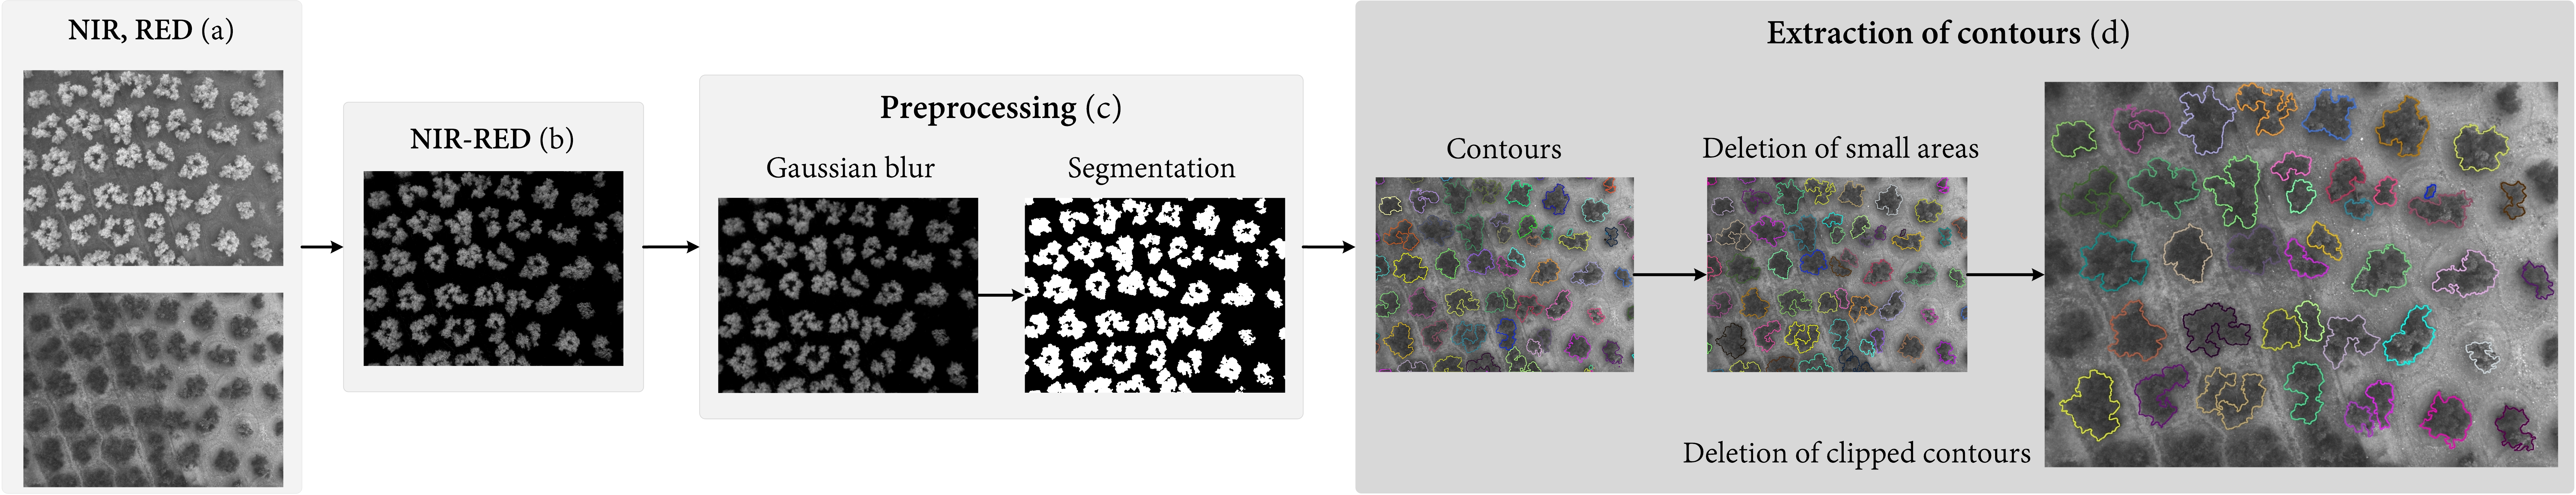
\includegraphics{figs/image_fusion/contour_retrieval.png}
	\caption{Processing of multispectral images to distinguish vegetation of interest from crop soil.}
	\label{fig:contour_extraction}
\end{figure*}

The proposed framework enables obtaining RGB, multispectral and thermographic data from a crop. Using some of these layers, it can also be applied to the temporal tracking of individual trees. More specifically, multispectral images are sensitive to vegetation and thus can help in the identification of trees. Once identified, points belonging to each one can be further analyzed to extract vegetation indices such as NDVI. 

The observed surface reflectance, $f(\theta)$, presents some peaks where the vegetation reflectance reaches a maximum value. The contrast among layers with higher and lower reflectance enables distinguishing soil and canopy. Despite not having more fine-grained samples of $f(\theta)$ as in hyperspectral data, relative maximum and minimum reflectance values concerning vegetation are visible at $\mathtt{NIR}$ and $\mathtt{RED}$ layers, respectively. Soil reflectance is assumed to be constant or small throughout all these layers, and thus can be easily filtered out. Therefore, $\mathtt{NIR}-\mathtt{RED}$ produces the result shown in Figure \ref{fig:contour_extraction}.

Besides the image difference, the following steps are previously performed:
\begin{enumerate}
    \item \textbf{Gaussian blur} to smooth the image colour and remove noise.
    \item \textbf{Image thresholding} to isolate the vegetation-labelled pixels.
    \item \textbf{Extracting a hierarchy of contours}. Contours within another are not of interest and therefore are discarded. Neither are of interest small contours belonging to low vegetation or noise, and cropped contours (partially visible). The latter can be identified since they have horizontal or vertical edges on the image boundaries.
\end{enumerate}

The identification of individual trees can be modulated using the size of a blur mask, the maximum area to be discarded and a threshold value high enough to avoid merging tree contours. Despite this method obtaining accurate contours, most of them contain hundreds of points and thus the polygon can be simplified by obtaining its convex hull \cite{sklansky_finding_1982} or other preferred polygons (e.g., hexagons). 

\begin{figure}[hbp]
    \centering
    \includegraphics[width=1\linewidth]{figs/image_fusion/convex_hull_contours.png}
    \caption{Conversion of tree contours into their convex hull and hexagons.}
    \label{fig:convex_hull_contours}
\end{figure}

\section{Validation}
\label{sec:image_fusion_evaluation}

This work has been evaluated with four different datasets depicting olive orchards located in Jaén, a Southern region of Spain. The first threee datasets have multispectral and RGB images, whereas the last collect RGB and thermal imagery. The main study area covers two hectares of olive trees in which the proposed methodology has been checked. Figure \ref{fig:image_fusion_study_area} presents a general overview of the main study area.

\begin{figure}[htb]
    \centering
    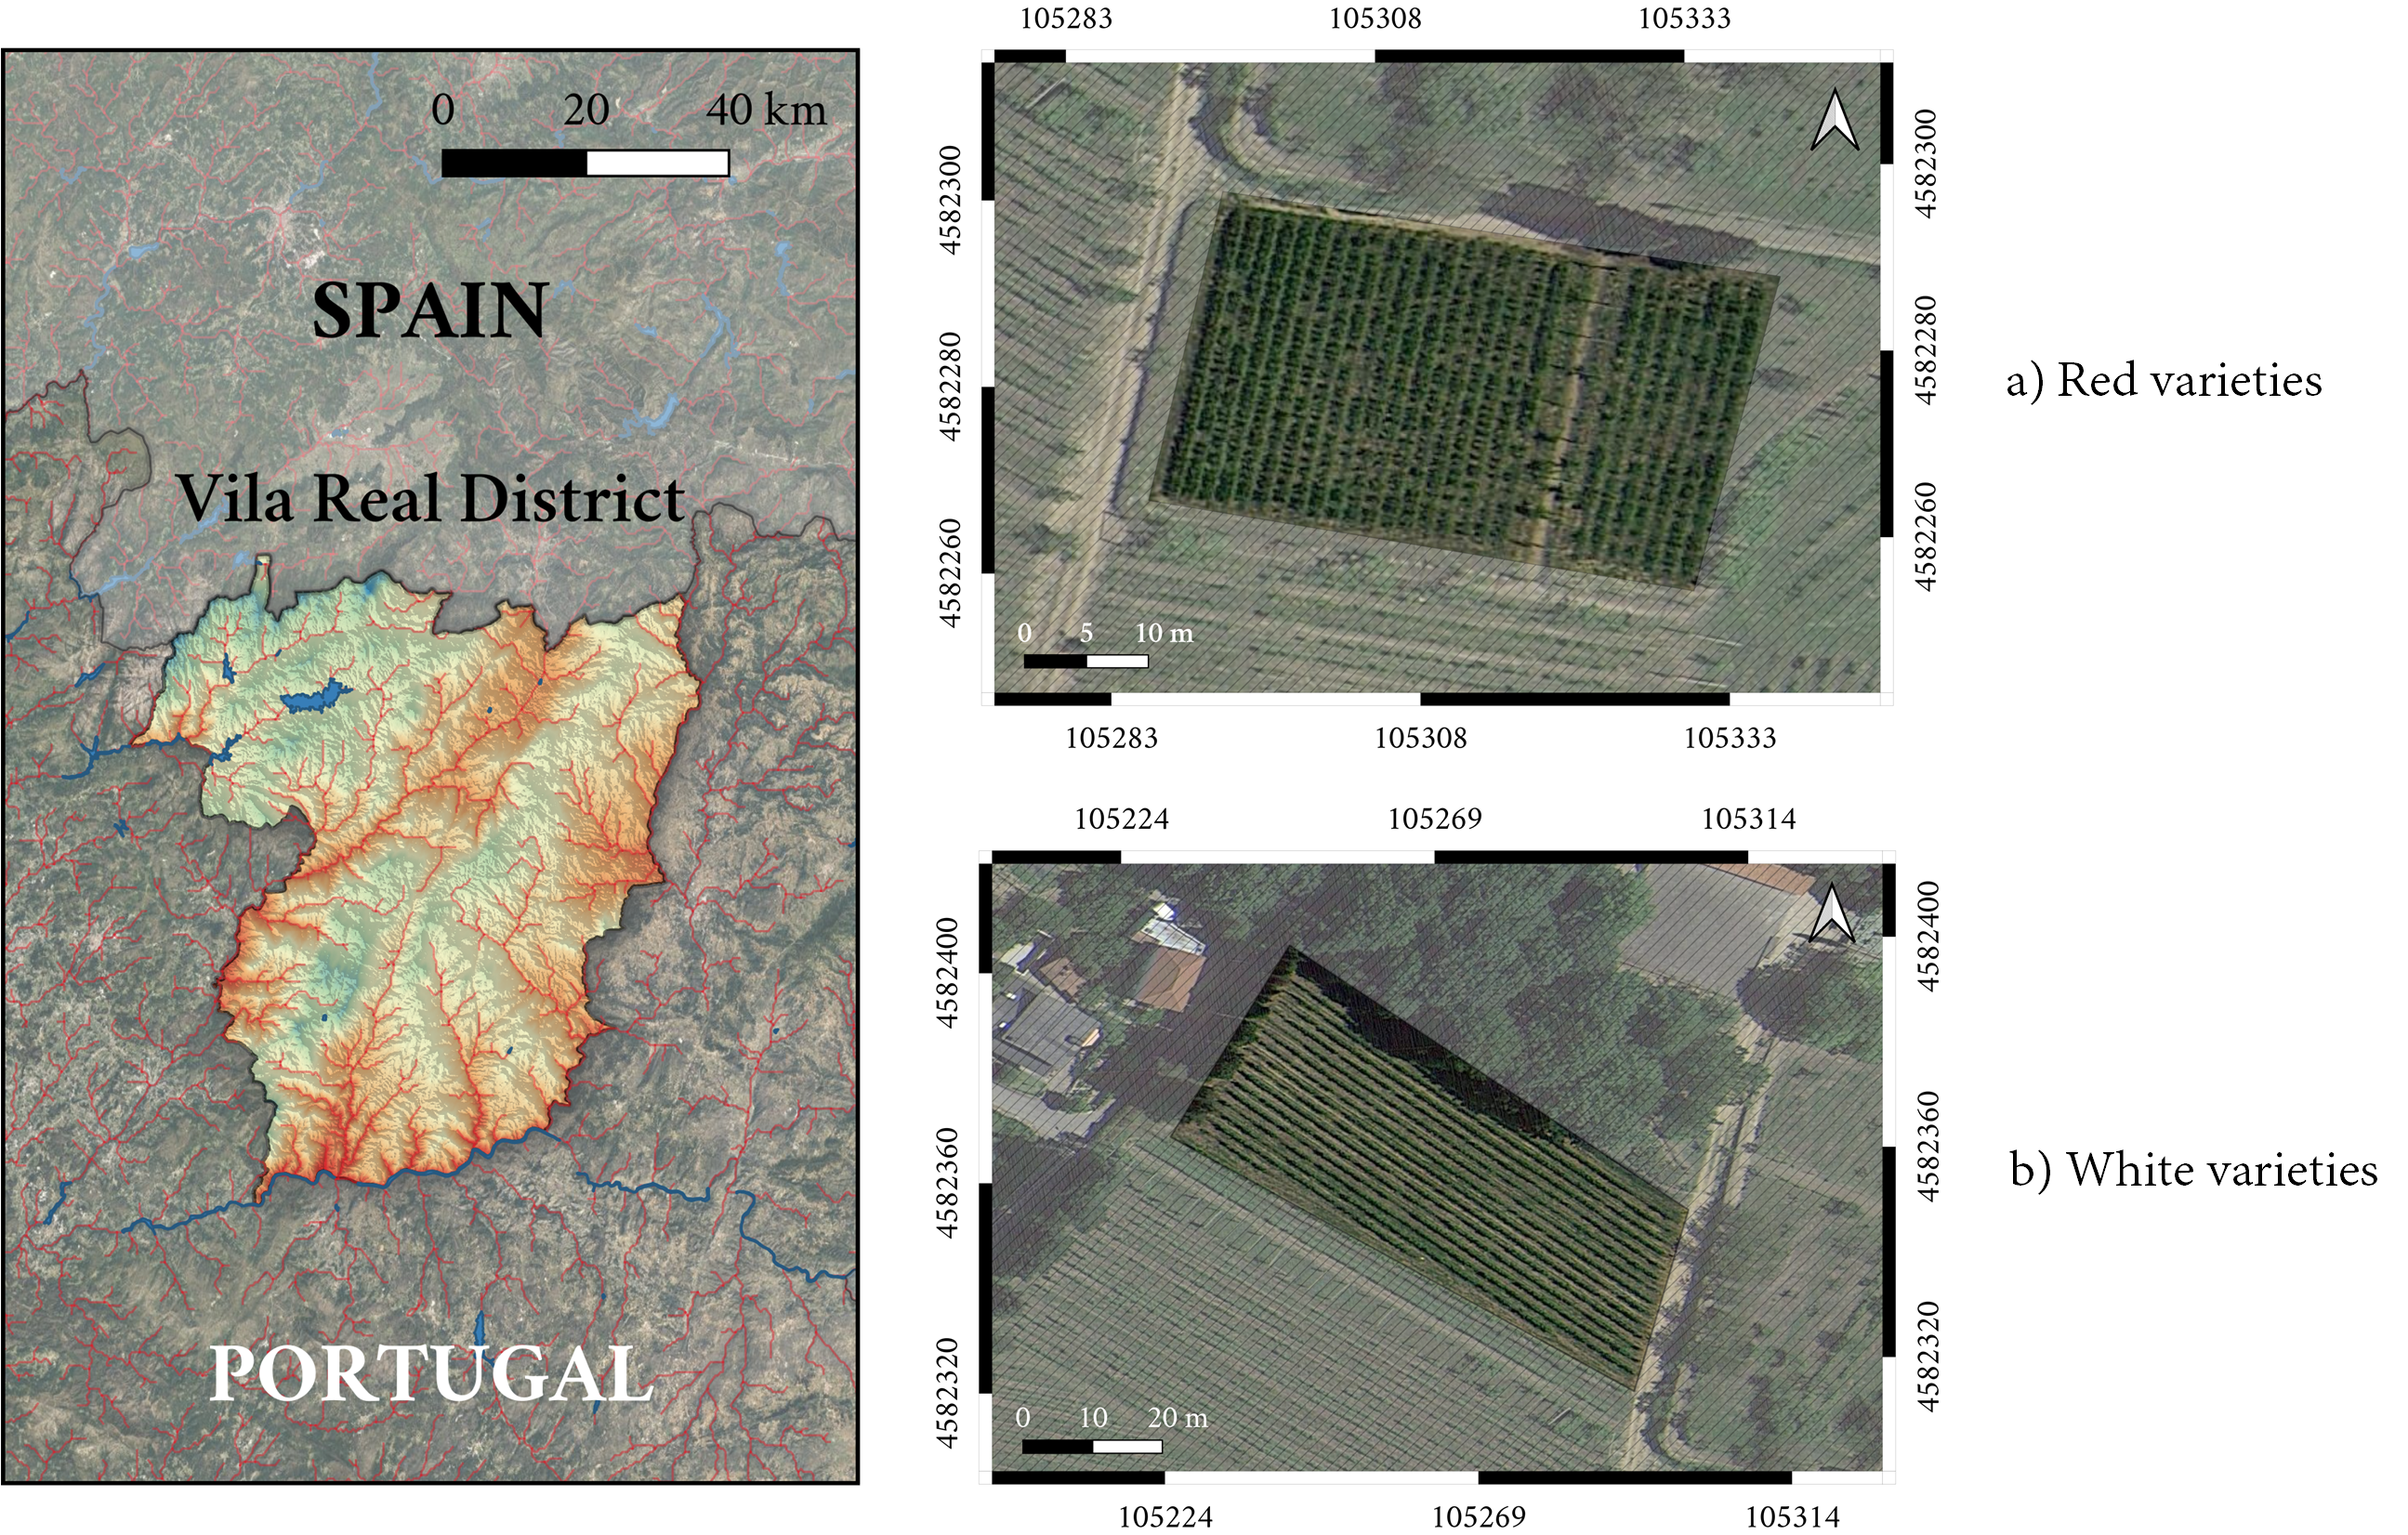
\includegraphics{figs/image_fusion/study_area.png}
    \caption{An overview of the study area. Coordinates are given in UTM (Universal Transverse Mercator) coordinate system.}
    \label{fig:image_fusion_study_area}
\end{figure}

The measurements were performed on a PC with Intel Core i7.6700 3.4GHz, 16GB RAM, NVIDIA GTX 1070 with 8GB RAM and Windows 10 OS. The implementation of the ECC algorithm was provided by the image processing library OpenCV within a C++ environment. The accuracy of the matching process was estimated using the normalized correlation coefficient (CC), defined as shown in Equation \ref{ec:correlationCoefficient}. The CC metric obtains a coefficient $\rho \in [0, 1]$ that measures the similarity between two images $I$ and $T$, source and template. It is a simple estimation measuring the intensity difference among images and therefore is not an exact measurement of the matching accuracy. Images to be compared were selected randomly from the four datasets.
\begin{equation}
    \label{ec:correlationCoefficient}
    \textit{CC} = \frac{\sum_{x',y'} T(x',y') * I(x + x', y + y')}{\sqrt{\sum_{x',y'}T(x',y')^{2} * \sum_{x',y'}I(x + x',y + y')^{2}}}
\end{equation}

Three parameters that affect the response time and registration accuracy were checked: 
\begin{itemize}
    \item \textbf{Precision to converge}. The closer it gets to zero, the harder is for the algorithm to converge.
    \item \textbf{Number of iterations}. Using a larger number of iterations may not improve the result since the algorithm can converge earlier.
    \item \textbf{Image size}. Smaller dimensionality may not obtain worse results and can help to decrease the response time and achieve faster convergence. 
\end{itemize}

\section{Results and discussion}
\label{sec:Results}

\textbf{Multispectral registration}. Four tests were launched to prove the accuracy of the registration methodology using the four multispectral bands. The original correlation coefficient is presented in Table \ref{table:multispectral_base_correlation} to highlight the improvement of the four matching tests against the first scenario. The dimensionality of multispectral images is low, and therefore, they do not need to be downscaled by default. The first set-up uses parameters that seem to be close to the optimal configuration, although the response time is higher. Table \ref{table:multispectral_rgb_correlation} shows that worse results for images that shows human-made objects due to a higher difference in the colour intensity. However, these are well aligned by visual inspection. The second test shows that the response time can be decreased at expense of lower CC. The third one uses an intermediate configuration that achieves high CC values with low latency. Finally, the fourth test downscales the image size by three, thus leading to higher CC with a lower response time. However, the latter returns worse results by visual inspection.

\renewcommand{\arraystretch}{1.2}
\begin{table}
    \captionsetup{singlelinecheck=off}
    \caption{Normalized correlation coefficient between original multispectral images. }
    \label{table:multispectral_base_correlation}
    \begin{tabular}{ll|c@{\hskip 0.5in}c@{\hskip 0.5in}c}
        \toprule
        & & \multicolumn{3}{c}{GRE} \\
        \cmidrule{1-5}
        & & RED & NIR & REG \\
        \cmidrule{1-5}
        Dataset & Viewpoint & $\rho$ & $\rho$ & $\rho$ \\
        \cmidrule{1-5}
        \multirow{3}{*}{1} & 1 & $0.8954$ & $0.8777$ & $0.9306$\\
        & 4 & $0.9777$ & $0.9381$ & $0.9618$\\
        & 6 & $0.9756$ & $0.9520$ & $0.9727$\\
        \cmidrule{1-5}
        \multirow{4}{*}{2} & 37 & $0.9286$ & $0.9100$ & $0.9371$\\
        & 48 & $0.9265$ & $0.8918$ & $0.9316$\\
        & 58 & $0.9146$ & $0.8878$ & $0.9242$\\
        & 53 & $0.9777$ & $0.9381$ & $0.9618$\\
        \cmidrule{1-5}
        \multirow{8}{*}{3} & 9 & $0.9669$ & $0.9545$ & $0.9714$\\
        & 35 & $0.9578$ & $0.9453$ & $0.9739$\\
        & 78 & $0.9707$ & $0.9504$ & $0.9672$\\
        & 107 & $0.9602$ & $0.9537$ & $0.9686$\\
        & 136 & $0.9755$ & $0.9612$ & $0.9692$\\
        & 141 & $0.9732$ & $0.9551$ & $0.9744$\\
        & 142 & $0.9728$ & $0.9375$ & $0.9656$\\
        & 144 & $0.9731$ & $0.9316$ & $0.9622$\\
        \cmidrule{1-5}
        \multicolumn{2}{r|}{\textbf{Average}} & \textbf{0.9564} & \textbf{0.9323} & \textbf{0.9581}\\
        \bottomrule
    \end{tabular}
\end{table}
\renewcommand{\arraystretch}{1}

\renewcommand{\arraystretch}{1.15}
\begin{table*}
    \caption{Normalized correlation coefficient and response time on the matching of a random subset of multispectral images over four different tests (test 1: $n \gets 30, p \gets 1\textsuperscript{-10}$, test 2: $n \gets 15, p \gets 1\textsuperscript{-2}$, test 3: $n \gets 15, p \gets 1\textsuperscript{-10}$ and test 4: $n \gets 150, p \gets 1\textsuperscript{-60}$).}
    \label{table:multispectral_correlation_registration}
    \begin{tabular}{ll|cccr|cccr}
        \toprule
        \multicolumn{2}{c}{} & \multicolumn{4}{c}{Test 1} & \multicolumn{4}{c}{Test 2}\\
        \cmidrule{1-10}
        & & \multicolumn{3}{c}{GRE} & & \multicolumn{3}{c}{GRE} & \\
        & & RED & NIR & REG & & RED & NIR & REG\\
        Dataset & Viewpoint & $\rho$ & $\rho$ & $\rho$ & \#time (\si{\second}) & $\rho$ & $\rho$ & $\rho$ & \#time (\si{\second}) \\
        \cmidrule{1-10}
        \multirow{3}{*}{1} & 1 & $0.9545$ & $0.9186$ & $0.9403$ & $3.627$ & $0.9545$ & $0.9181$ & $0.9395$ & $1.128$\\
        & 4 & $0.9888$ & $0.9473$ & $0.9681$ & $3.576$ & $0.9814$ & $0.9473$ & $0.9681$ & $950$\\
        & 6 & $0.9861$ & $0.9591$ & $0.9772$ & $3.622$ & $0.9817$ & $0.9591$ & $0.9767$ & $1.079$\\
        \cmidrule{1-10}
        \multirow{4}{*}{2} & 48 & $0.9654$ & $0.9107$ & $0.9368$ & $3.580$ & $0.9654$ & $0.9107$ & $0.9368$ & $1.282$\\
        & 58 & $0.9546$ & $0.9088$ & $0.9321$ & $3.607$ & $0.9547$ & $0.9088$ & $0.9321$ & $1.224$\\
        & 53 & $0.9888$ & $0.9473$ & $0.9681$ & $3.573$ & $0.9814$ & $0.9473$ & $0.9681$ & $955$\\
        & 37 & $0.9628$ & $0.9265$ & $0.9461$ & $3.569$ & $0.9463$ & $0.9265$ & $0.9460$ & $1.100$\\
        \cmidrule{1-10}
        \multirow{8}{*}{3} & 35 & $0.9973$ & $0.9654$ & $0.9785$ & $3.543$ & $0.9973$ & $0.9645$ & $0.9766$ & $1.090$\\
        & 107 & $0.9973$ & $0.9621$ & $0.9776$ & $3.558$ & $0.9973$ & $0.9621$ & $0.9776$ & $1.356$\\
        & 136 & $0.9973$ & $0.9677$ & $0.9767$ & $3.577$ & $0.9781$ & $0.9623$ & $0.9760$ & $581$\\
        & 78 & $0.9957$ & $0.9640$ & $0.9731$ & $3.575$ & $0.9956$ & $0.9615$ & $0.9696$ & $1.353$\\
        & 142 & $0.9962$ & $0.9632$ & $0.9749$ & $3.567$ & $0.9772$ & $0.9632$ & $0.9748$ & $989$\\
        & 144 & $0.9964$ & $0.9580$ & $0.9715$ & $3.586$ & $0.9781$ & $0.9580$ & $0.9715$ & $994$\\
        & 9 & $0.9967$ & $0.9713$ & $0.9810$ & $3.585$ & $0.9967$ & $0.9713$ & $0.9810$ & $1.471$\\
        & 141 & $9966$ & $0.9746$ & $0.9791$ & $3.518$ & $0.9967$ & $0.9713$ & $0.9810$ & $1.110$\\
        \cmidrule{1-10}
        \multicolumn{2}{r|}{\textbf{Average}} & \textbf{0.9849} & \textbf{0.9496} & \textbf{0.9654} & \textbf{3577.53} & \textbf{0.9788} & \textbf{0.9488} & \textbf{0.965} & \textbf{1110.8}\\
        \bottomrule
    \end{tabular}
\end{table*}
\renewcommand{\arraystretch}{1}

\renewcommand{\arraystretch}{1.15}
\begin{table*}
    \captionsetup{singlelinecheck=off}
    \caption{Continuation of Table \ref{table:multispectral_correlation_registration}.}
    \begin{tabular}{ll|cccr|cccr}
        \toprule
        \multicolumn{2}{c}{} & \multicolumn{4}{c}{Test 3} & \multicolumn{4}{c}{Test 4}\\
        \cmidrule{1-10}
        & & \multicolumn{3}{c}{GRE} & & \multicolumn{3}{c}{GRE} & \\
        & & RED & NIR & REG & & RED & NIR & REG\\
        Dataset & Viewpoint & $\rho$ & $\rho$ & $\rho$ & \#time (\si{\second}) & $\rho$ & $\rho$ & $\rho$ & \#time (\si{\second}) \\
        \cmidrule{1-10}
        \multirow{3}{*}{1} & 1 & $0.9545$ & $0.9186$ & $0.9403$ & $1.933$ & $0.9540$ & $0.9181$ & $0.9394$ & $1.797$\\
        & 4 & $0.9866$ & $0.9474$ & $0.9682$ & $1.900$ & $0.9883$ & $0.9473$ & $0.9665$ & $1.780$\\
        & 6 & $0.9838$ & $0.9592$ & $0.9772$ & $1.927$ & $0.9849$ & $0.9610$ & $0.9767$ & $1.818$\\
        \cmidrule{1-10}
        \multirow{4}{*}{2} & 48 & $0.9654$ & $0.9107$ & $0.9367$ & $1.884$ & $0.9651$ & $0.9113$ & $0.9368$ & $1.746$\\
        & 58 & $0.9546$ & $0.9088$ & $0.9321$ & $1.994$ & $0.9651$ & $0.9113$ & $0.9368$ & $1.774$\\
        & 53 & $0.9866$ & $0.9474$ & $0.9682$ & $1.921$ & $0.9883$ & $0.9473$ & $0.9665$ & $1.760$\\
        & 37 & $0.9628$ & $0.9265$ & $0.9461$ & $1.895$ & $0.9618$ & $0.9266$ & $0.9455$ & $1.774$\\
        \cmidrule{1-10}
        \multirow{8}{*}{3} & 35 & $0.9973$ & $0.9654$ & $0.9785$ & $1.905$ & $0.9972$ & $0.9659$ & $0.9778$ & $1.805$\\
        & 107 & $0.9973$ & $0.9621$ & $0.9776$ & $1.920$ & $0.9970$ & $0.9618$ & $0.9762$ & $1.788$\\
        & 136 & $0.9966$ & $0.9645$ & $0.9766$ & $1.900$ & $0.9969$ & $0.9671$ & $0.9752$ & $1.761$\\
        & 78 & $0.9957$ & $0.9640$ & $0.9731$ & $1.903$ & $0.9948$ & $0.9633$ & $0.9714$ & $1.798$\\
        & 142 & $0.9941$ & $0.9632$ & $0.9749$ & $1.909$ & $0.9961$ & $0.9632$ & $0.9740$ & $1.773$\\
        & 144 & $0.9909$ & $0.9580$ & $0.9715$ & $1.898$ & $0.9963$ & $0.9580$ & $0.9702$ & $1.774$\\
        & 9 & $0.9967$ & $0.9713$ & $0.9810$ & $1.911$ & $0.9964$ & $0.9713$ & $0.9806$ & $1.789$\\
        & 141 & $9966$ & $0.9746$ & $0.9791$ & $1.873$ & $0.9965$ & $0.9750$ & $0.9786$ & $1.789$\\
        \cmidrule{1-10}
        \multicolumn{2}{r|}{\textbf{Average}} & \textbf{0.9839} & \textbf{0.9493} & \textbf{0.9654} & \textbf{1904.86} & \textbf{0.9852} & \textbf{0.9499} & \textbf{0.9648} & \textbf{1781.73}\\
        \bottomrule
    \end{tabular}
\end{table*}
\renewcommand{\arraystretch}{1}

\textbf{RGB and multispectral registration}. Table \ref{table:multispectral_rgb_correlation} shows the results of three different tests. Intensity differences between images are higher and therefore, the response time increases. The second test obtains the lowest latency, while the first achieves the same result with increased response time. This scenario proves the convergence of the ECC algorithm; the safest approach selects a large value that guarantees the ECC convergence, whereas a real-time application may opt for a lower number of iterations at expense of risking the convergence. Both tests use images with a size equal to the multispectral dimensionality split by two. Such size enables smoothing the image and improving the registration process, despite a small blur still being required. The third test uses the starting multispectral size and RGB images are downscaled to fit them. It returns worse results than previous tests since the number of iterations and precision are reduced to avoid high execution times. 

\renewcommand{\arraystretch}{1.15}
\begin{table*}
    \caption{Normalized correlation coefficient and response time on the matching of a random subset of multispectral and RGB images (test 1: $d \gets \textit{multispectral}_{\textit{size}} / 2, n \gets 400, p \gets 1\textsuperscript{-60}$, test 2: $d \gets \textit{multispectral}_{\textit{size}} / 2, n \gets 150, p \gets 1\textsuperscript{-30}$ and test 3: $d \gets \textit{multispectral}_{\textit{size}}, n \gets 100, p \gets 1\textsuperscript{-20}$).}
    \label{table:multispectral_rgb_correlation}
    \begin{tabular}{ll|cc|cc|cc}
        \toprule
        \multicolumn{2}{c}{} & \multicolumn{2}{c}{Test 1} & \multicolumn{2}{c}{Test 2} & \multicolumn{2}{c}{Test 3}\\
        \cmidrule{1-8}
        Dataset & Viewpoints & $\rho$ & \#time (\si{\second}) & $\rho$ & \#time (\si{\second}) & $\rho$ & \#time (\si{\second})\\
        \cmidrule{1-8}
        \multirow{5}{*}{4} & 1, 916 & $0.9683$ & $8.090$ & $0.9683$ & $2.810$ & $0.9569$ & $7.405$\\
        & 148, 918 & $0.9664$ & $7.882$ & $0.9664$ & $2.839$ & $0.9408$ & $7.022$\\
        & 142, 904 & $0.9711$ & $7.506$ & $0.9711$ & $2.757$ & $0.9453$ & $7.058$\\ 
        & 137, 892 & $0.9761$ & $7.221$ & $0.9761$ & $2.718$ & $0.9747$ & $7.448$\\
        & 144, 906 & $0.9690$ & $7.266$ & $0.9690$ & $2.724$ & $0.9680$ & $7.087$\\
        \cmidrule{1-8}
        \multicolumn{2}{r|}{\textbf{Average}} & \textbf{0.9701} & \textbf{7593} & \textbf{0.9701} & \textbf{2769.6} & \textbf{0.9571} & \textbf{7204}\\
        \bottomrule
    \end{tabular}
\end{table*}
\renewcommand{\arraystretch}{1}

\textbf{Thermal and RGB registration}. Three tests were proposed with the same parameters as before (Table \ref{table:thermal_rgb_correlation}). In comparison with previous tests, size reduction does not have a great impact since contours are smoothed out in thermal images. CC values were also lower than in previous tests since the registration results have areas with undetermined values, as shown in Figure \ref{fig:thermal_comparative}. Therefore, the first and third tests show the outcome of downscaling the starting thermal size. Both reach the best CC, whereas the third returns the same results as the first with lower latency due to the convergence. The second test uses the starting thermal size and obtains almost the same CC average at the cost of a slightly higher response time. In contrast with multispectral tests, the first and third set-ups use smaller dimensionality but do not obtain inaccurate matches by visual inspection. In conclusion, using the original size is not needed in this case. 

\section{Conclusions}

A framework for registering heterogeneous UAV-based images into a multi-layer model was proposed. The ECC algorithm was applied to this task, thus showing it is highly suitable for matching images in different spectral wavelengths. Through a case study, we have also proposed a method to identify individual trees using multispectral images, which can be further used in multi-temporal tracking applied to crops.

The differences between aerial images are typically smaller than in terrestrial images, and yet affine transformations have been necessary. From this framework, an adaptive process starting from a reduced size and scaling up to the original size could be proposed. Reducing the size helps in finding an approximate transformation with a lower response time, which could be used in the estimation of an initial, yet large, transformation. On the other hand, estimations with larger image sizes enable optimizing the result. 

\renewcommand{\arraystretch}{1.15}
\begin{table*}[t]
    \caption{Normalized correlation coefficient and response time on the matching of a random subset of RGB and thermal images over three different tests (test 1: $d \gets \textit{thermal}_{\textit{size}} / 2, n \gets 300, p \gets 1\textsuperscript{-60}$, test 2: $d \gets \textit{thermal}_{\textit{size}}, n \gets 100, p \gets 1\textsuperscript{-20}$ and test 3: $d \gets \textit{thermal}_{\textit{size}} / 2, n \gets 60, p \gets 1\textsuperscript{-20}$).}
    \label{table:thermal_rgb_correlation}
    \begin{tabular}{ll|cr|cr|cr}
        \toprule
        \multicolumn{2}{c}{} & \multicolumn{2}{c}{Test 1} & \multicolumn{2}{c}{Test 2} & \multicolumn{2}{c}{Test 3}\\
        \toprule
        Dataset & Viewpoint & $\rho$ & \#time (\si{\second}) & $\rho$ & \#time (\si{\second}) & $\rho$ & \#time (\si{\second})\\
        \cmidrule{1-8}
        \multirow{8}{*}{3} & 394 & $0.9756$ & $2.779$ & $0.9771$ & $3.204$ & $0.9756$ & $1.419$\\
        & 626 & $0.9728$ & $2.834$ & $0.9745$ & $3.320$ & $0.9728$ & $1.389$\\
        & 726 & $0.9728$ & $2.951$ & $0.9741$ & $3.211$ & $0.9728$ & $1.411$\\ 
        & 928 & $0.9756$ & $2.761$ & $0.9770$ & $3.341$ & $0.9756$ & $1.401$\\
        & 467 & $0.9416$ & $2.731$ & $0.9385$ & $3.134$ & $0.9417$ & $1.381$\\
        & 643 & $0.9511$ & $2.789$ & $0.9494$ & $3.137$ & $0.9511$ & $1.404$\\ 
        & 963 & $0.9444$ & $2.881$ & $0.9425$ & $3.177$ & $0.9444$ & $1.403$\\
        & 475 & $0.9396$ & $2.946$ & $0.9358$ & $3.257$ & $0.9396$ & $1.390$\\
        \cmidrule{1-8}
        \multirow{4}{*}{4} & 922 & $0.9674$ & $2.791$ & $0.9690$ & $3200$ & $0.9674$ & $1.396$\\
        & 554 & $0.9786$ & $2.790$ & $0.9803$ & $3.267$ & $0.9786$ & $1.402$\\
        & 405 & $0.9266$ & $2.716$ & $0.9265$ & $3.187$ & $0.9266$ & $1.400$\\
        & 607 & $0.9511$ & $2.794$ & $0.9502$ & $3.236$ & $0.9511$ & $1.382$\\
        \cmidrule{1-8}
        \multicolumn{2}{r|}{\textbf{Average}} & \textbf{0.9581} & \textbf{2813.58} & \textbf{0.9579} & \textbf{3222.58} & \textbf{0.9581} & \textbf{1398.16}\\
        \bottomrule
    \end{tabular}
\end{table*}
\renewcommand{\arraystretch}{1}

